\documentclass[conference]{IEEEtran}
\IEEEoverridecommandlockouts
% The preceding line is only needed to identify funding in the first footnote. If that is unneeded, please comment it out.
\usepackage{cite}
\usepackage{amsmath,amssymb,amsfonts}
\usepackage{algorithmic}
\usepackage{graphicx}
\usepackage{textcomp}
\usepackage{xcolor}
\usepackage[utf8]{inputenc}
\def\BibTeX{{\rm B\kern-.05em{\sc i\kern-.025em b}\kern-.08em
    T\kern-.1667em\lower.7ex\hbox{E}\kern-.125emX}}
\begin{document}

\title{Trabalho 1 AC 3}

\author{\IEEEauthorblockN{1\textsuperscript{st} Rafael Augusto Barros Ladeira de Oliveira}
\IEEEauthorblockA{\textit{PUC Minas ICEI (Instituto de Ciências Exatas e Informática)} \\
\textit{Pontifical Catholic University of Minas Gerais (PUC Minas)}\\
Belo Horizonte, Minas Gerais, Brazil \\
rafael@theancientscroll.com}
\and
\IEEEauthorblockN{2\textsuperscript{nd} Henrique Mendonça Castelar Campos}
\IEEEauthorblockA{\textit{PUC Minas ICEI (Instituto de Ciências Exatas e Informática)} \\
\textit{Pontifical Catholic University of Minas Gerais (PUC Minas)}\\
Belo Horizonte, Minas Gerais, Brazil \\
henriquemendonacastelar@gmail.com}
}

\maketitle

\section{abstract}
The purpose of this article is to test the performance of a MIPS processor according to it’s specifications, which includes the size of the cache memory, the algorithm for replacing the data in the cache memory and the size of the cache line. For that, a program called Amnesia was used, a memory hierarchy simulator of a MIPS processor.\footnote{The program Amnesia can be download on this address: http://amnesia.lasdpc.icmc.usp.br/amnesia-en/}
%\Latex{abstract}

\begin{IEEEkeywords}
Amnesia, MIPS, Memory Hierarchy, Simulator, Replacement Algorithm, Computer Ar.
\end{IEEEkeywords}

\section{Introdução}
Um dos grande desafios da indústria dos microprocessadores é aumentar a performance de seus chips. Um dos fatores que interferem significativamente no desempenho de um microprocessador em um computador é a sua hierarquia de memória, que dependendo das configurações, pode aumentar ou diminuir o tempo necessário para acessar os dados que serão processados, o que poderá resultar em um alto ou baixo desempenho. Visando a entender um padrão que leve a um melhor desempenho, vários testes foram realizados no software Amnesia.

\section{Testes Realizados no Amensia}
O Amnesia é um projeto de Paulo Lopes e Sarita Bruschi, com a finalidade de ajudar alunos de engenharia da computação e derivados¸ a entender melhor hierarquia de memória de hardware computacional, para fins educacionais. Com ele estudantes e educadores simulam a atitude de diferentes registradores e processadores variando a memória cache, memoria virtual e paginada dos mesmos em diferentes cenários utilizando traces, instruções de acesso, leitura e .

Em cada teste realizado foi utilizada uma configuração diferente na máquina. Todos os testes rodaram o mesmo programa.

\subsection{Alteração dos Algoritmos de Substituição de Dados na Memoria Cache}

Durante os testes foi alternado entre os algoritmos de substituição de dados na memória cache. Os algoritmos utilizados foram o LRU (Least recently used) e o FIFO (First in first out). O LRU substitui o dado que foi menos recentemente utilizado, enquanto que o FIFO remove os dados na ordem em que eles foram inseridos.

\subsection{Alteração do Tamanho da Memória Cache}

Nos testes foram testado processadores com diferentes tamanhos de memória cache. O tamanho foi variado entre 8, 16 e 32 Bytes. Na teoria, quanto maior for o tamanho da memória cache menor será a taxa de não acertos (cache miss) o que resulta em um melhor desempenho. 

\subsection{Alteração do Tamanho da Linha da Memória Cache}

Nas configurações foram utilizados diferentes tamanhos de linha de memória cache. Os tamanhos variam entre 2, 4, 8 e 16 Bytes.

\subsection{Funcionamento do Amnesia}

\begin{figure}
  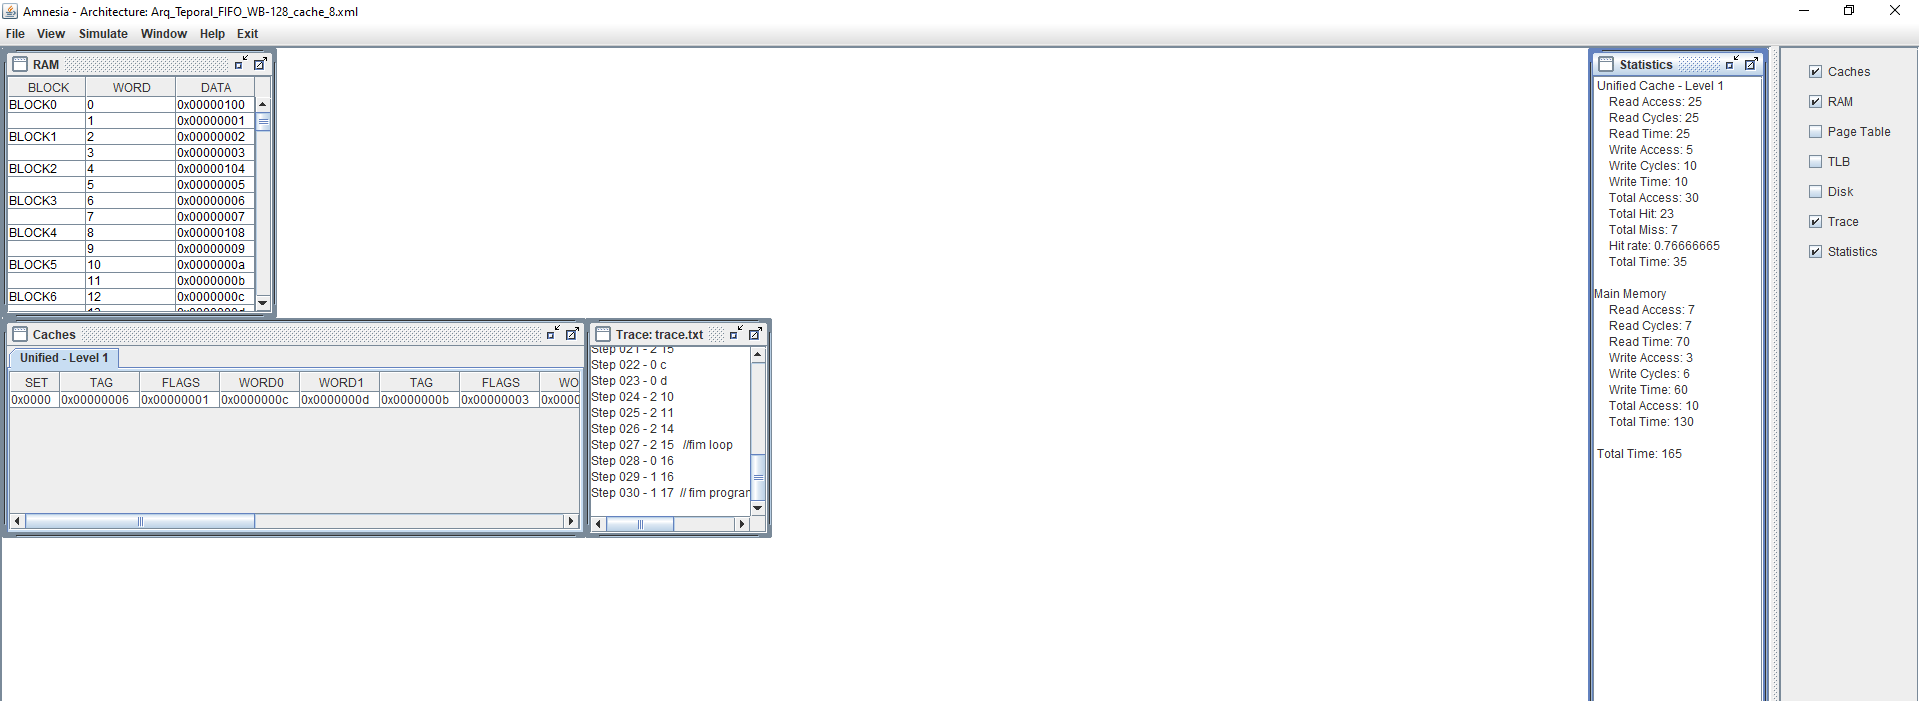
\includegraphics[width=\linewidth]{Amnesia_screen.png}
  \caption{Tela do Programa Amnesia fazendo um teste}
  \label{fig:boat1}
\end{figure}

\begin{itemize}
\item  
Geral . \\ \\
O simulador nos permite gerar diferentes cenários de simulações de liteura e escrita de dados
customizando as configurações de hierarquia de mémoria a partir da alteração de diversas configurações da memoria. Exemplo FIFO ou LRU e seu memory size, cache size e line size dentre outros. Além disso podemos testar diversos cenáriso diferentes para uma mesma memória e como ela se comportaria para os varios cenários criados para testar suas capacidades, quando incluimos os mesmos no programa apartir dos seus arquivos traces. Logo, uma simulação nunca tera os mesmos resultados.\\
\\
\item Traces. \\
Os arquivos traces são  arquivos normalmente na extensão txt contendo as instruções de acesso que serão realizadas pela nossa arquitetura de memoria da simulação no prograama Amnesia. Neles as ações são divididas em 5 tipos de instruções. Onde as de rótulo 0 executam a leitura de dados, 1 gravação de dados, 2 busca de instrução, 3 registro escape(tratado como tipo de acesso desconhecido) e por ultímo a 4 que é registro escape(operação cache de flush)
Apartir dos chamados traces criamos instruções para testar as capacidades dos processadores. Onde o 
\
\end{itemize}

\section{Resultados dos Testes}

\begin{figure}
    \centering
    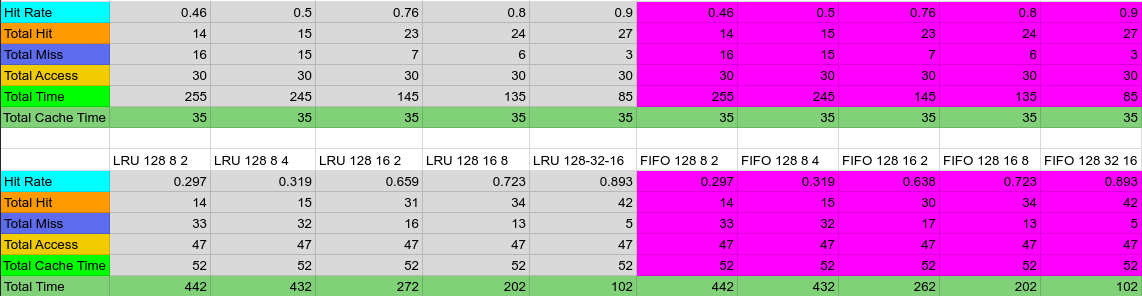
\includegraphics[width=\linewidth]{Imagens/Tabela.png}
    \caption{Comparação das taxas de acerto entre FIFO e LRU.\\Na tabela de cima a memória virtual está desabilitada. Já na tabela de baixo a memória virtual está habilitada}
    \label{fig:Comparação das taxas de acerto entre FIFO e LRU.\\Na tabela de cima a memória virtual está desabilitada. Já na tabela de baixo a memória virtual está habilitada}
\end{figure}

\begin{figure}
    \centering
    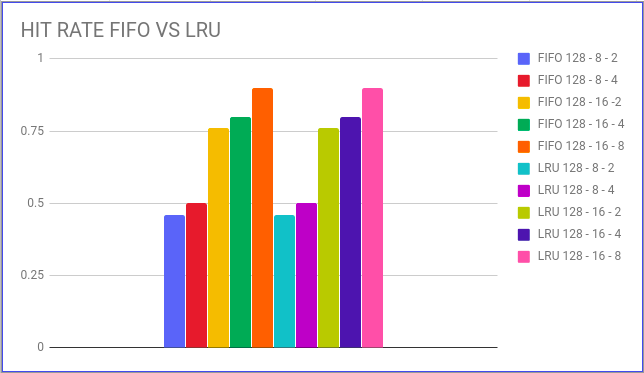
\includegraphics[width=\linewidth]{Imagens/Hit_RATE_FIFO_VS_LRU.png}
    \caption{Taxa de acerto na memória cache em FIFO vs LRU}
    \label{fig:Taxa de acerto na memória cache em FIFO vs LRU}
\end{figure}

\begin{figure}
    \centering
    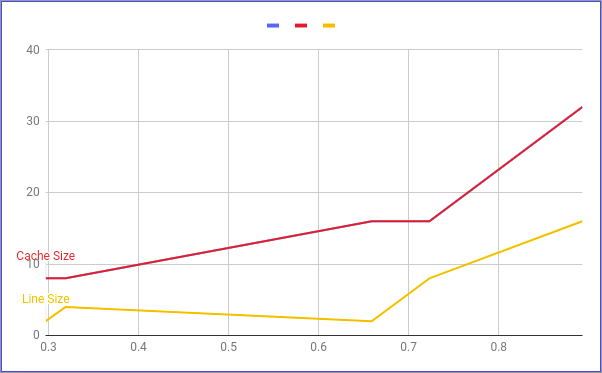
\includegraphics[width=\linewidth]{Imagens/WRITE_TIME_POR_HIT_RATE.png}
    \caption{Tempo de escrita por taxa de acerto na memória cache}
    \label{fig:Tempo de escrita por taxa de acerto na memória cache}
\end{figure}

\begin{figure}
    \centering
    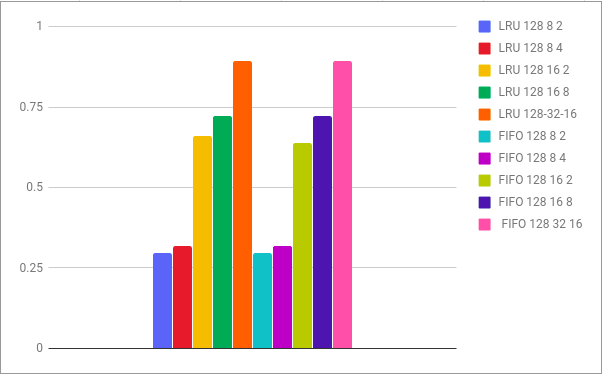
\includegraphics[width=\linewidth]{Imagens/HIT_RATE_POR_ARQUITETURA.png}
    \caption{Taxa de acerto por arquitetura}
    \label{fig:Taxa de acerto por arquitetura}
\end{figure}

Na comparação da taxa de acertos na memória cache não houve diferença significativa entre a política de substituição FIFO e LRU.

\section{Conclusão}

\section{Referências Bibliográficas}




{\BibTeX} does not work by magic. It doesn't get the bibliographic
data from thin air but from .bib files. If you use {\BibTeX} to produce a
bibliography you must send the .bib files. 

{\LaTeX} can't read your mind. If you assign the same label to a
subsubsection and a table, you might find that Table I has been cross
referenced as Table IV-B3. 

{\LaTeX} does not have precognitive abilities. If you put a
\verb|\label| command before the command that updates the counter it's
supposed to be using, the label will pick up the last counter to be
cross referenced instead. In particular, a \verb|\label| command
should not go before the caption of a figure or a table.

Do not use \verb|\nonumber| inside the \verb|{array}| environment. It
will not stop equation numbers inside \verb|{array}| (there won't be
any anyway) and it might stop a wanted equation number in the
surrounding equation.

\subsection{Some Common Mistakes}\label{SCM}
\begin{itemize}
\item The word ``data'' is plural, not singular.
\item The subscript for the permeability of vacuum $\mu_{0}$, and other common scientific constants, is zero with subscript formatting, not a lowercase letter ``o''.
\item In American English, commas, semicolons, periods, question and exclamation marks are located within quotation marks only when a complete thought or name is cited, such as a title or full quotation. When quotation marks are used, instead of a bold or italic typeface, to highlight a word or phrase, punctuation should appear outside of the quotation marks. A parenthetical phrase or statement at the end of a sentence is punctuated outside of the closing parenthesis (like this). (A parenthetical sentence is punctuated within the parentheses.)
\item A graph within a graph is an ``inset'', not an ``insert''. The word alternatively is preferred to the word ``alternately'' (unless you really mean something that alternates).
\item Do not use the word ``essentially'' to mean ``approximately'' or ``effectively''.
\item In your paper title, if the words ``that uses'' can accurately replace the word ``using'', capitalize the ``u''; if not, keep using lower-cased.
\item Be aware of the different meanings of the homophones ``affect'' and ``effect'', ``complement'' and ``compliment'', ``discreet'' and ``discrete'', ``principal'' and ``principle''.
\item Do not confuse ``imply'' and ``infer''.
\item The prefix ``non'' is not a word; it should be joined to the word it modifies, usually without a hyphen.
\item There is no period after the ``et'' in the Latin abbreviation ``et al.''.
\item The abbreviation ``i.e.'' means ``that is'', and the abbreviation ``e.g.'' means ``for example''.
\end{itemize}
An excellent style manual for science writers is \cite{b7}.

\subsection{Authors and Affiliations}
\textbf{The class file is designed for, but not limited to, six authors.} A 
minimum of one author is required for all conference articles. Author names 
should be listed starting from left to right and then moving down to the 
next line. This is the author sequence that will be used in future citations 
and by indexing services. Names should not be listed in columns nor group by 
affiliation. Please keep your affiliations as succinct as possible (for 
example, do not differentiate among departments of the same organization).

\subsection{Identify the Headings}
Headings, or heads, are organizational devices that guide the reader through 
your paper. There are two types: component heads and text heads.

Component heads identify the different components of your paper and are not 
topically subordinate to each other. Examples include Acknowledgments and 
References and, for these, the correct style to use is ``Heading 5''. Use 
``figure caption'' for your Figure captions, and ``table head'' for your 
table title. Run-in heads, such as ``Abstract'', will require you to apply a 
style (in this case, italic) in addition to the style provided by the drop 
down menu to differentiate the head from the text.

Text heads organize the topics on a relational, hierarchical basis. For 
example, the paper title is the primary text head because all subsequent 
material relates and elaborates on this one topic. If there are two or more 
sub-topics, the next level head (uppercase Roman numerals) should be used 
and, conversely, if there are not at least two sub-topics, then no subheads 
should be introduced.

\subsection{Figures and Tables}
\paragraph{Positioning Figures and Tables} Place figures and tables at the top and 
bottom of columns. Avoid placing them in the middle of columns. Large 
figures and tables may span across both columns. Figure captions should be 
below the figures; table heads should appear above the tables. Insert 
figures and tables after they are cited in the text. Use the abbreviation 
``Fig.~\ref{fig}'', even at the beginning of a sentence.

\begin{table}[htbp]
\caption{Table Type Styles}
\begin{center}
\begin{tabular}{|c|c|c|c|}
\hline
\textbf{Table}&\multicolumn{3}{|c|}{\textbf{Table Column Head}} \\
\cline{2-4} 
\textbf{Head} & \textbf{\textit{Table column subhead}}& \textbf{\textit{Subhead}}& \textbf{\textit{Subhead}} \\
\hline
copy& More table copy$^{\mathrm{a}}$& &  \\
\hline
\multicolumn{4}{l}{$^{\mathrm{a}}$Sample of a Table footnote.}
\end{tabular}
\label{tab1}
\end{center}
\end{table}

\begin{figure}[htbp]
\centerline{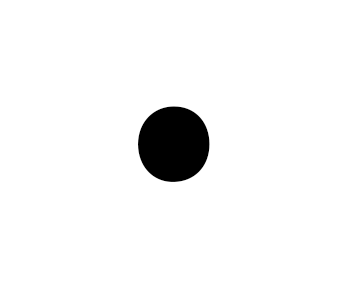
\includegraphics{fig1.png}}
\caption{Example of a figure caption.}
\label{fig}
\end{figure}

Figure Labels: Use 8 point Times New Roman for Figure labels. Use words 
rather than symbols or abbreviations when writing Figure axis labels to 
avoid confusing the reader. As an example, write the quantity 
``Magnetization'', or ``Magnetization, M'', not just ``M''. If including 
units in the label, present them within parentheses. Do not label axes only 
with units. In the example, write ``Magnetization (A/m)'' or ``Magnetization 
\{A[m(1)]\}'', not just ``A/m''. Do not label axes with a ratio of 
quantities and units. For example, write ``Temperature (K)'', not 
``Temperature/K''.

\section*{Acknowledgment}

The preferred spelling of the word ``acknowledgment'' in America is without 
an ``e'' after the ``g''. Avoid the stilted expression ``one of us (R. B. 
G.) thanks $\ldots$''. Instead, try ``R. B. G. thanks$\ldots$''. Put sponsor 
acknowledgments in the unnumbered footnote on the first page.

\section*{Referencias}

Please number citations consecutively within brackets \cite{b1}. The 
sentence punctuation follows the bracket \cite{b2}. Refer simply to the reference 
number, as in \cite{b3}---do not use ``Ref. \cite{b3}'' or ``reference \cite{b3}'' except at 
the beginning of a sentence: ``Reference \cite{b3} was the first $\ldots$''

Number footnotes separately in superscripts. Place the actual footnote at 
the bottom of the column in which it was cited. Do not put footnotes in the 
abstract or reference list. Use letters for table footnotes.

Unless there are six authors or more give all authors' names; do not use 
``et al.''. Papers that have not been published, even if they have been 
submitted for publication, should be cited as ``unpublished'' \cite{b4}. Papers 
that have been accepted for publication should be cited as ``in press'' \cite{b5}. 
Capitalize only the first word in a paper title, except for proper nouns and 
element symbols.

For papers published in translation journals, please give the English 
citation first, followed by the original foreign-language citation \cite{b6}.

\begin{thebibliography}{00}
\bibitem{b1} G. Eason, B. Noble, and I. N. Sneddon, ``On certain integrals of Lipschitz-Hankel type involving products of Bessel functions,'' Phil. Trans. Roy. Soc. London, vol. A247, pp. 529--551, April 1955.
\bibitem{b2} J. Clerk Maxwell, A Treatise on Electricity and Magnetism, 3rd ed., vol. 2. Oxford: Clarendon, 1892, pp.68--73.
\bibitem{b3} I. S. Jacobs and C. P. Bean, ``Fine particles, thin films and exchange anisotropy,'' in Magnetism, vol. III, G. T. Rado and H. Suhl, Eds. New York: Academic, 1963, pp. 271--350.
\bibitem{b4} K. Elissa, ``Title of paper if known,'' unpublished.
\bibitem{b5} R. Nicole, ``Title of paper with only first word capitalized,'' J. Name Stand. Abbrev., in press.
\bibitem{b6} Y. Yorozu, M. Hirano, K. Oka, and Y. Tagawa, ``Electron spectroscopy studies on magneto-optical media and plastic substrate interface,'' IEEE Transl. J. Magn. Japan, vol. 2, pp. 740--741, August 1987 [Digests 9th Annual Conf. Magnetics Japan, p. 301, 1982].
\bibitem{b7} M. Young, The Technical Writer's Handbook. Mill Valley, CA: University Science, 1989.
\end{thebibliography}
\vspace{12pt}
\color{red}
IEEE conference templates contain guidance text for composing and formatting conference papers. Please ensure that all template text is removed from your conference paper prior to submission to the conference. Failure to remove the template text from your paper may result in your paper not being published.

\end{document}
